The simplest solution to measure the performance in a recall focused IR task is to evaluate the recall, however, it fails to reflect how early a system retrieves the relevant documents. Although recall is the objective for such applications, the score should be able to distinguish between systems that retrieve relevant documents earlier than those that retrieve them later. For recall-oriented IR applications, the problem is viewed as a ranking problem with a cut-off for a maximum number of documents to be checked $ N_{max} $.\\\\
\textbf{Patent Retrieval Evaluation Score}
\ \\
Patent retrieval evaluation score (PRES)~\citep{magdy2010pres} is a novel metric for evaluating recall-oriented IR applications, which derived from the normalised recall measure ($ R_{norm} $). It measures the ability of a system to retrieve all known relevant documents earlier in the ranked list. Unlike MAP and Recall, PRES is dependent on the relative effort exerted by users to find relevant documents. This is mapped by $ N_{max} $ (Equation \ref{eq:pres}), which is an adjustable parameter that can be set by users and indicates the maximum number of documents they are willing to check in the ranked list. PRES measures the effectiveness of ranking documents relative to the best and worst ranking cases, where the best ranking case is retrieving all relevant documents at the top of the list, and the worst is to retrieve all the relevant documents just after the maximum number of documents to
be checked by the user ($ N_{max} $). The idea behind this assumption is that getting any relevant document after $ N_{max} $ leads to it being missed by the user, and getting all relevant documents after max leads to a zero recall, which is the theoretical worst case scenario. 
%Figure 1 shows an illustrative graph of how to calculate PRES, where 
PRES is the area between the actual and worst cases ($ A_{2} $) divided by the area between the best and worst cases ($ A_{1}+A_{2} $).
$ N_{max} $ introduces a new definition to the quality of ranking of relevant results, as the ranks of results are relative to the value of $ N_{max} $. For example, getting a relevant document at the rank 10 will be very good when $ N_{max}=1000 $, good when $ N_{max}=100 $, but bad when $ N_{max}=15 $, and very bad when $ N_{max}=10 $. Systems with a higher recall can achieve a lower PRES value when compared to systems with a lower recall but a better average ranking. The PRES value varies from $ R $ to $ \frac{nR^{2}}{N_{max}} $, where $ R $ is the recall, according to the average quality of ranking of relevant documents.
\begin{figure}[htpb]
   \centering
%   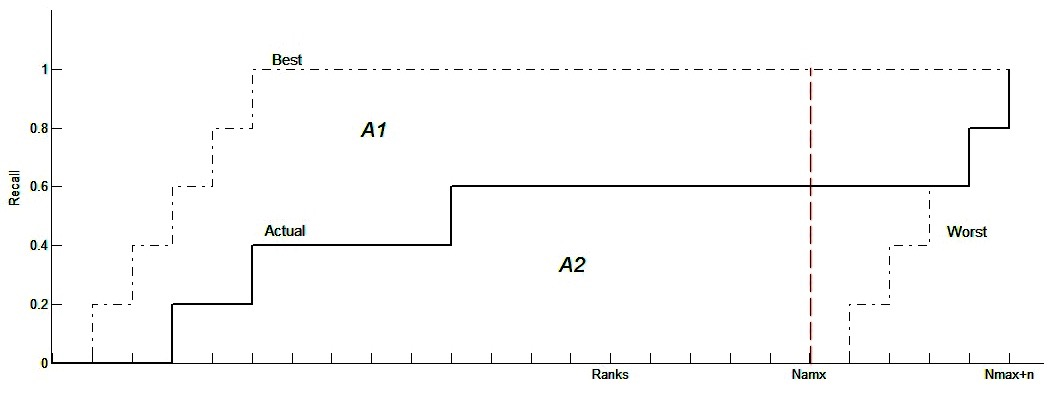
\includegraphics[width=1\textwidth,height=50mm]{figs/pres.jpg}
   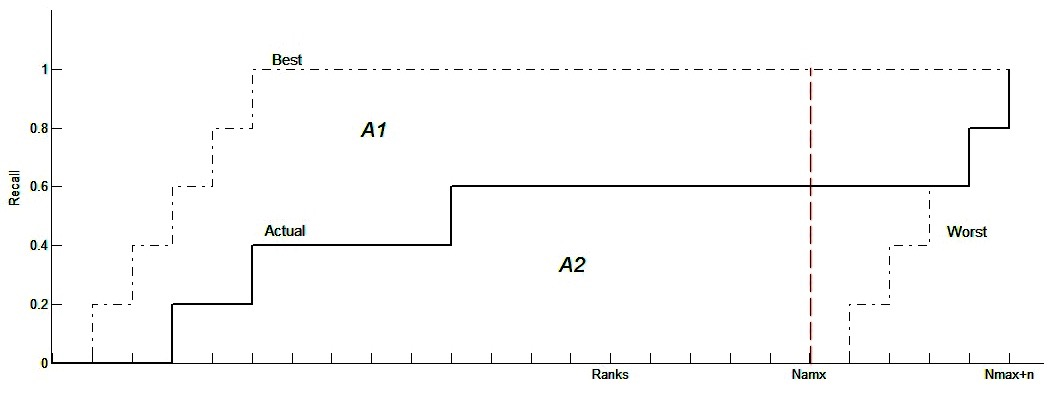
\includegraphics[scale=.37]{figs/pres.jpg}
   \caption{PRES curve is bounded between the best case and the new defined worst case~\citep{magdy2010pres}.}  
   \label{fig:pres} 
\end{figure}
\FloatBarrier 
\begin{equation}
\label{eq:pres}
PRES=\frac{A_{2}}{A_{1}+A_{2}}=1-\frac{\frac{\sum r_{i}}{n}-\frac{n+1}{2}}{N_{max}},
\end{equation}
where $ r_{i} $ is the rank at which the $ i $th relevant document is retrieved, $ N_{max} $ is the maximum number of retrieved documents to be checked by the user (i.e. the cut-off number of retrieved documents) and $ n $ is the total number of relevant documents.